\documentclass[tikz, border=0.15mm]{standalone}
\usepackage{ytableau,tikz,varwidth}
\usetikzlibrary{calc}
\usepackage{mathrsfs}
\newcommand{\typeA}{magenta!65}
\newcommand{\typeB}{blue!75}
\newcommand{\typeC}{green!65}

\begin{document}
\ytableausetup{mathmode, boxframe=normal, boxsize=2.5em}
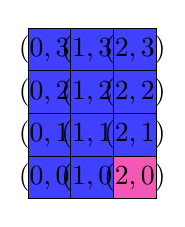
\begin{tikzpicture}[inner sep=0in,outer sep=0in]
	\node (n) {\begin{varwidth}{5cm}{
				\begin{ytableau}
					*(\typeB) (0,3) & *(\typeB) (1,3) & *(\typeB) (2,3) \\
					*(\typeB) (0,2) & *(\typeB) (1,2) & *(\typeB) (2,2) \\
					*(\typeB) (0,1) & *(\typeB) (1,1) & *(\typeB) (2,1) \\
					*(\typeB) (0,0) & *(\typeB) (1,0) & *(\typeA) (2,0) \\
			\end{ytableau}}\end{varwidth}};
	%\draw[thick, black, -stealth] (n.south west)--([xshift=0.4cm]n.south east);
	%\node[xshift = 0.60cm] at (n.south east) {$\mathscr{T}_1$};
	
	%\draw[thick, black, -stealth] (n.south west)--([yshift=0.4cm]n.north west);
	%\node[yshift = 0.55cm] at (n.north west) {$\mathscr{T}_2$};
\end{tikzpicture}
\end{document}